\chapter{Toward Low Power}
In this chapter, we introduce a recently developed low-power router. We start by illustrating the motivation of advancing to low power system. Then we present the design and how it is tested in SBN context.

\section{Motivation}
As pointed out in section \ref{challenges}, photovoltaic system is intensively adopted in SBN due to poor or non-existing power supply. The choice of battery is critical in designing an effecient PV system. Within the context of SBN, most batteries available at local market are lead-acid batteries intended for cars and motors, more commonly known as "starting battery". They are designed to supply a large current for a short time to start engine, instead of being deeply discharged with mild current.

In a photovoltaic system, the battery can only be charged during daytime, and may be drained generously with heavy load over night. Deep discharges shorten cycle life of these batteries due to sulfation and crystalization. Elevated internal resistance also makes charging harder. Hence, deep cycle batteries are preferred in PV systems. Unfortunately they are not widely available in Tanzania and come with a relatively higher price.

To prolong the life of starting batteries in PV systems, deep discharges should be avoided by either expanding battery capacity (using a larger battery) or reducing load (drawing less energy from batteries). Given capacity of battery $C(Ah)$, output voltage of battery $V$, power consumption $P(watt)$ and discharging time $t$, Depth of Discharge (DoD) can be denoted as:
\begin{equation}
DoD = \frac{Pt}{CV}
\end{equation}

Table \ref{power_consumptions} shows the power consumption of several typical equipments in SBN. Table \ref{dod} reveals the approximate depth of discharge (DoD) of 100Ah and 50Ah batteries for 16 hours\footnote{A PV system in Serengeti area can effectively accept solar power for 7~8 hours a day, which leaves approximately 16 hours with battery as the only power source.} under various power consumptions.

\begin{table}\label{power_consumptions}
\centering
\begin{tabular}{cc}
\hline
Device & Power Consumption \\
\hline
Cisco 2950 series switch & 30W \\
Supermicro X7SPA Montherboard & 14W \\
Ubiquiti Nanostation & 8W \\
Odroid U2 & 5W \\
\hline
\end{tabular}
\caption{Power consumptions of frequently used equipments in SBN}
\end{table}

\begin{table}\label{dod}
\centering
\begin{tabular}{c|cc}
\hline
 & 50Ah & 100Ah \\
\hline
40W & Over-discharged & 53.3\% \\
30W & 80\% & 40 \% \\
20W & 53\% & 26.7\% \\
10W & 26.7\% & 13.3\% \\
\hline
\end{tabular}
\caption{Depth of Discharge for different batteries under different load}
\end{table}

Adding batteries leads to more investment and more labor work for mantenance. Thus, we strive to the lower power consumption ($watt$) while meeting the demand of capacity ($bps$).  

\section{System Design}\label{sysdesign}
In the initial phase of SBN, connection on fiber-optic line is enabled by Cisco 2950 series switch with fiber-optic SFP ports\footnote{http://www.cisco.com/c/en/us/products/switches/catalyst-2950-series-switches/index.html}. An inverter with multiple power input is used to connect DC from power grid, battery and switch. The drawbacks of this design are clear:
\begin{itemize}
\item The whole system is energy-hungry, given high power consumption of switch and low efficiency of inverter.
\item There is a lack of cut-off voltage protection for batteries.
\item Significant room is consumed to store these equipments.
\end{itemize}

Our low-power optical fibre router design includes a motherboard, network interface card(s)(NIC) which supports one or more optical SFP ports and integrated charge controller. The montheboard of first generation router includes following components:
\begin{itemize}
\item Motherboard: Intel/ATOM-based Supermicro X7SA, supporting PCIe I/O-bus.
\item NIC: Interface master Niagara 82048, providing four GIGA SFP ports with digital optical monitoring.
\end{itemize}
The idling power consumption of the Motherboard is 14W and for the NIC 8W. The differences between idling and full-load is negligible. A bandwidth of 1Gbps is fulfilled in this design, although the power consumption is still not optimal according to Table \ref{dod}, especially when distribution radio is taken into consideration. We refer this version as Supermicro router.

To further minimize power consumption while maintaining satisfactory bandwidth, a new version of low-power router is developed with following components:
\begin{itemize}
\item Motherboard: Odroid U3\footnote{http://www.hardkernel.com/main/products/prdt\_info.php?g\_code=g138745696275} with Arm-based Exynos4412 Quad-core processor.
\item NIC: one 10/100Mbps Ethernet with RJ45 pack. Two fibergecko 100 card\footnote{http://www.lyconsys.com/download/datasheet\_fibergecko100\_eng.pdf} with 100/1000Mbps SFP port and USB2.0 on I/O-bus.
\end{itemize}
We refer this version as Odroid-router. A comparison of Supermicro router and Odroid router is shown in Figure \ref{routers}.

\begin{figure}[htbp]
\centering
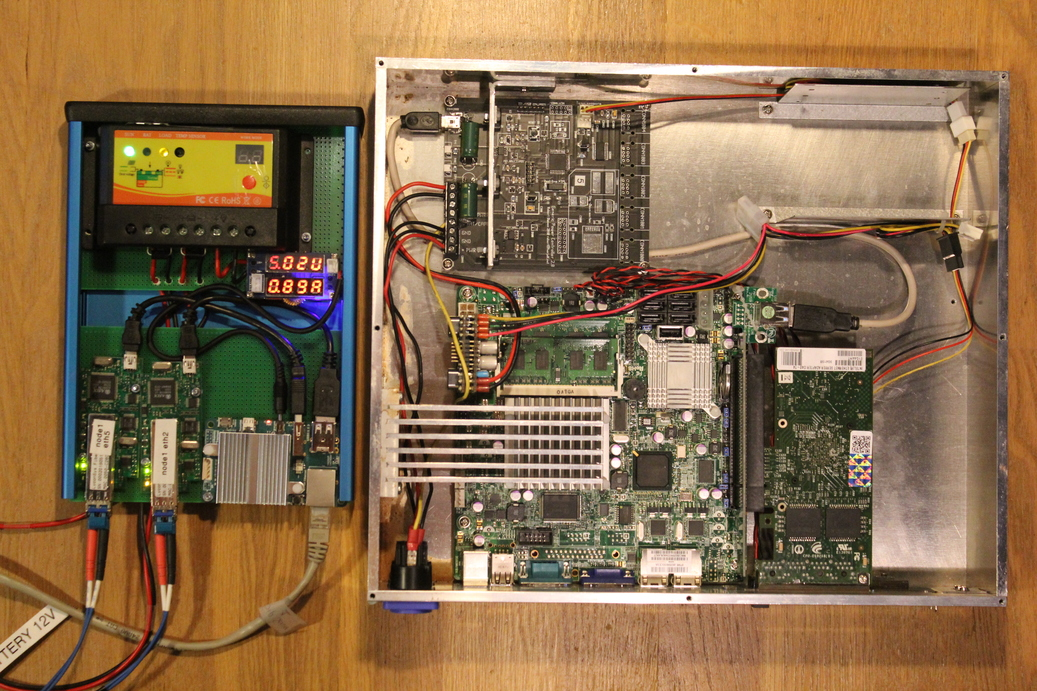
\includegraphics[width=0.6\textwidth]{routers.jpg}
\caption{The first generation low-power router to the right and the second to the left}
\label{routers}
\end{figure}

The power consumption of new design is approximately 5W and the difference between idling and full-load is negligible. The power consumption is significantly reduced with a compromise of bandwdith. The downgrade of speed is actually forced by the bottleneck of USB2.0 port as the I/O-bus. Local loop-back in the Exynos4412 quad-core processor reveals a communication capacity of 5Gbps. On the other hand, USB3.0 adds a new transfer mode "SuperSpeed" which is capable of tranferring data at up to 5Gbps. Hence, the possibility of upgrading the service back to 1Gbps or higher is promised, given capable motherboard and NIC cards.

The choice of motherboard is based on a benchmark of several candidates listed in Table \ref{candidates}. The benchmark is conducted using LMBench toolset\footnote{http://www.bitmover.com/lmbench/} and the result is revealed in Figure \ref{benchmark}. Packet forwarding is essentially based on table lookup, whose performance is impacted by memory latency and bandwidth. The lower latency and the higher bandwidth, the better. They are presented perspectively in the top and middle diagram of Figure \ref{benchmark}.

\begin{table}[htbp]
\centering
\begin{tabular}{c|ccc}
\hline
 & CPU Freq & Size ($mm\times mm$) & Weight \\
\hline
Raspberry Pi B & 0.7GHz & $85.6\times 56.5$ & 45g \\
Supermicro X7SPA & 1.8GHz & $170.2\times 170.2$ & \\
Odroid U3 & 1.7GHz & $83.0\times 48.0$ & 48g \\
Alix 2d3 & 0.5GHz & $152.4\times 152.4$ & \\
BeagleBone Black & 1.0GHz & $86.4\times 53.3$ & 40g \\
\hline
\end{tabular}
\caption{A list of router motherboard candidates}
\label{candidates}
\end{table}

\begin{figure}[htbp]
\centering
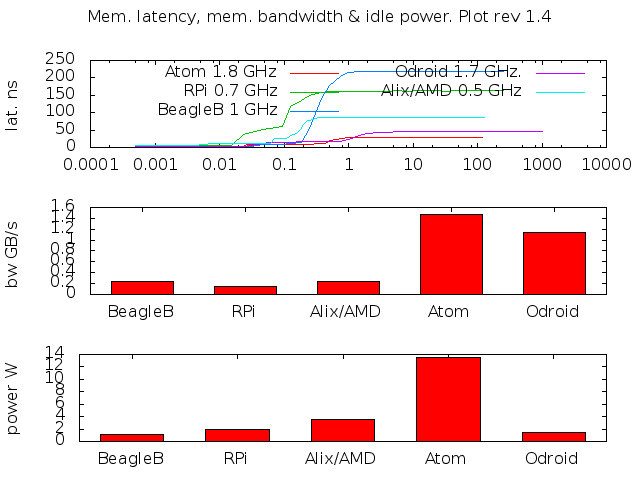
\includegraphics[width=\textwidth]{benchmark.jpg}
\caption{A benckmark of five low power platforms (top: memory latency; middle: memory bandwidth; bottom: idling power consumption}
\label{benchmark}
\end{figure}

Intel/ATOM-based system has the lowest memory latency although the data of Odroid comes very close to it. As for memory bandwidth, ATOM system is still the best, which is followed closely by Odroid. 

The idle power consumption in the bottom plot is measured without NICs. The Atom system consumes ~14W, the Alix board ~3.5W and other three platforms consume ~1.4W, about 10\% of Atom system. When adding two NICs to Odroid, the total power consumption becomes 4.57W when idling and 5.25W when fully loaded by forwarding  at speed of 95Mbps.

The result becomes clear by comparing five platforms that Atom system has the best performance in terms of memory latency and bandwidth, although followed closely by Odroid with significantly reduced power consumption. Odroid is also smaller in size and weight.

The operating system used previously in Supermicro router is Bifrost Linux distribution\footnote{http://bifrost.slu.se/}. A customized Debian-based distribution with added network performance test utilities is used in Odroid router.

\section{Deployment and Testing}
\subsection{Temperature Profiling at Nata site}
To further investigate the overheating problem addressed in Section \ref{challenges} and verify the proposal of burying batteries underground, wireless sensors\footnote{http://herjulf.se/products/WSN/sensors/} are deployed according to the diagram shown in Figure \ref{temperature_profile}

\begin{figure}[h]
\centering
\begin{subfigure}{0.45\textwidth}
\centering
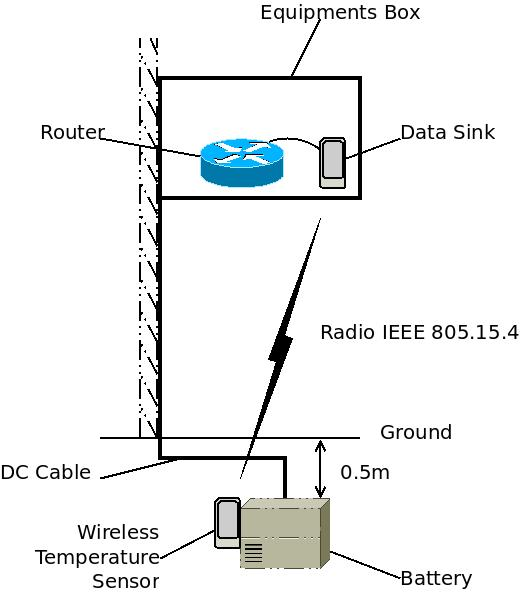
\includegraphics[width=\textwidth]{temp_test_diagram.jpeg}
\caption{Setup to profile ambient temperature}
\end{subfigure}
\begin{subfigure}{0.30\textwidth}
\centering
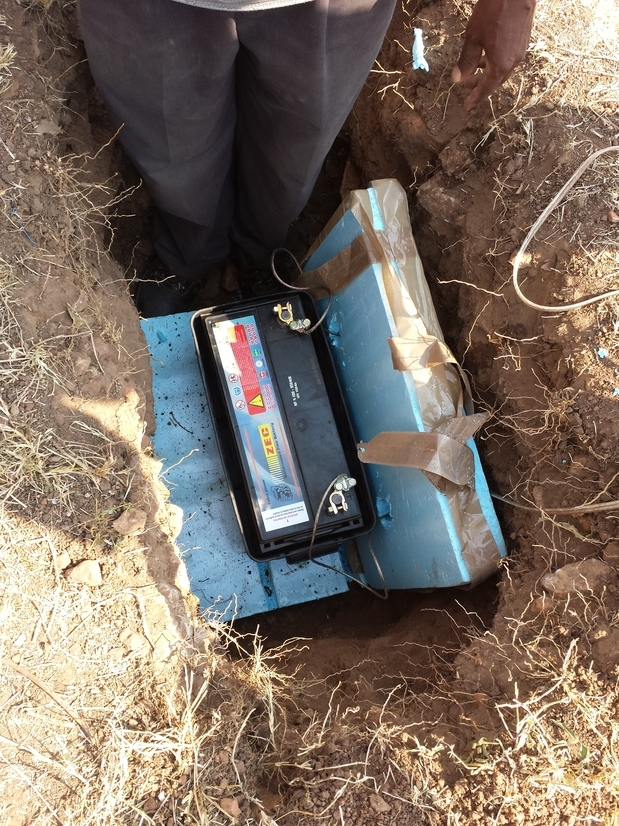
\includegraphics[width=\textwidth]{bury_bat.jpg}
\caption{Burying battery at Nata site}
\end{subfigure}
\caption{Temperature Profiling at Serengeti Nata site}
\label{temperature_profile}
\end{figure}

A wireless sensor node is buried along with a 100Ah battery. The sensor draws negligible current directly from battery and periodically report temperature data to sink node via IEEE 802.15.4. The sink node then send data to listening daemon running in low power router, in which data is accumulated for further analysis. With collected data, we plot temperature trend of 6 days at Nata site, see Figure \ref{temp_nata}.

\begin{figure}[h]
\centering
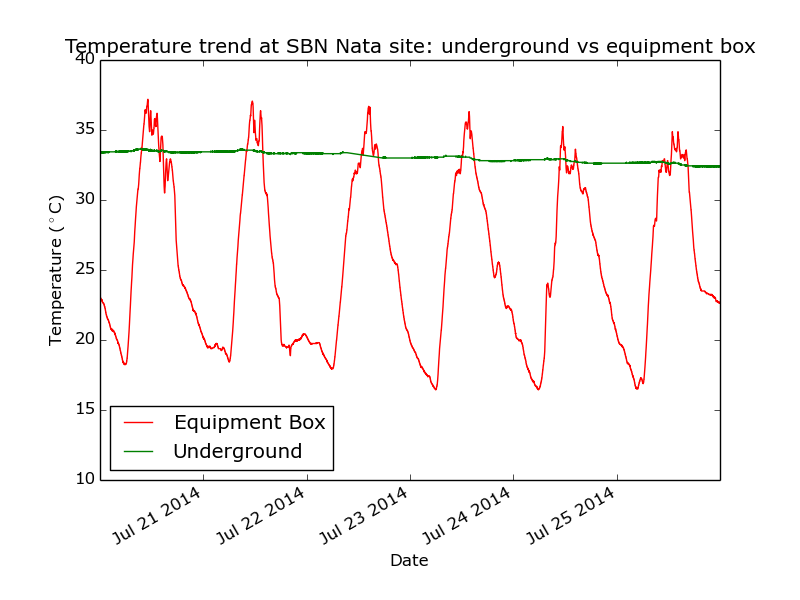
\includegraphics[width=0.8\textwidth]{temp_nata.png}
\caption{Temperature trend at Nata}
\label{temp_nata}
\end{figure}

The temperature in the equipment box is consistent with our observation. In addition, average temperatures are considerably uniform thourghout the whole year in Serengeti area. Hence, battery life can be prolonged if stored elsewhere cooler. However, temperatures under earth contradict with our expectation. Rather than stabling at 25\celsius\cite{jager1982soils}, temperature at 0.5m below surface stays at a constant level of 33\celsius. 

Hence, other approaches to bring down the battery temperature are yet to be further explored.

\subsection{Network Topology and Setup}
To test Odroid routers, three of them are deployed at Bunda, Nata and Mugumu sites respectively, along with Supermicro routers that are in service. The new topology after adding those routers is shown in Figure \ref{odroid_topology}. A subnet of 41.93.124.144/28 is allocated for testing.

\begin{figure}[h]
\centering
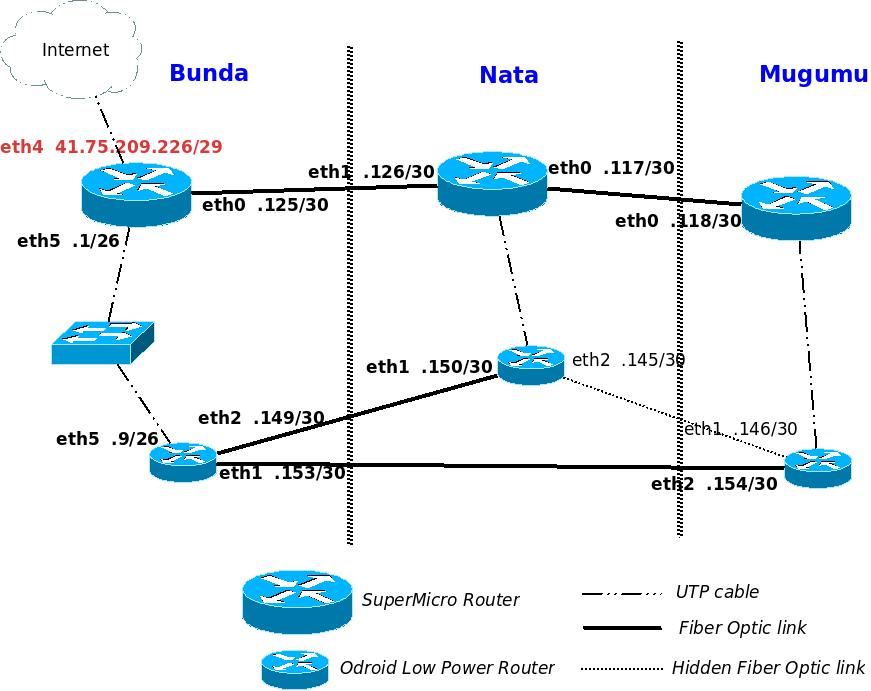
\includegraphics[width=\textwidth]{odroid_topology.jpeg}
\caption{Topology with odroid routers}
\label{odroid_topology}
\end{figure}

As introduced in Section \ref{sbn_intro}, SBN fiber line is comprised of two segments: Bunda-to-Nata and Nata-to-Mugumu, respectively. In previous setting, two segments are linked by the Supermicro router at Nata. As a result, this router becomes the single-point-of-failure (SPOF), whose failure causes disconnections of both Nata and Mugumu network. To eliminate the SPOF, it is proposed to have a fiber trand bypassing Nata, which links Bunda and Mugumu directly. Following restrictions need to be considered:
\begin{itemize}
\item The optical fiber line is poorly installed and only few of them are usable.
\item Even though necessary information is partially documented\footnote{RESEARCH AND DEVELOPMENT PROJECT ON INFORMATION AND COMMUNICATION TECHNOLOGY FOR RURAL DEVELOPMENT (ICT4RD) IN TANZANIA - Optical Fiber Commissioning Report Serengeti Site}. For single mode fiber, power loss of 0.5dBm/km for 1310nm is expected and 0.4dBm/km for 1550nm. The distances of two segments are 89km and 45km, which indicate \~45dBm power loss between Bunda and Nata, and \~22dBm loss between Nata and Mugumu. According to the documentation, fiber loss is less than that prediction, although abrupt discontinuities result in much power loss and noise observed at the end. In addition, power budget of SFP transceivers on Supermicro router is limited and could not tolerate the power loss combined. Thus, it is hard to bypass Nata with Supermicro routers.
\item Without proper tools, locating those fiber trands and testing are non-trivial and time-consuming tasks, especially at remote sites where the fiber spans over one hundred kilometers.
\end{itemize}
%TODO SFP transceiver model
%TODO appendix: how the fiber is connected
We use duplex SFP transceivers with higher power budget to reduce the number of fiber trands needed and to compensate for power loss. We are able to achieve a toplogy shown in Figure \ref{odroid_topology}. How fibers are wired is documented in Appendix X. To be noted, all the IP addresses in this diagram are within the subnet of 41.93.124.0/24, unless  labelled otherwise. For example, eth5 .1/26 indicates an IP address of 41.93.124.1/26 on NIC eth5. Routes are statically configured, for routing program is currently not enabled.

Odroid router comes with complete power supply circuit, as well as Supermicro router. Figure \ref{wiring} depicts how solar panel and battery are wired. Low Voltage Disconnect (LVD) level of Odroid router charge controller is set to be slightly lower than that of Supermicro router, and results in later shutdown of Odroid router when battery being exhausted.
\begin{figure}[h]
\centering
\begin{subfigure}{0.45\textwidth}
\centering
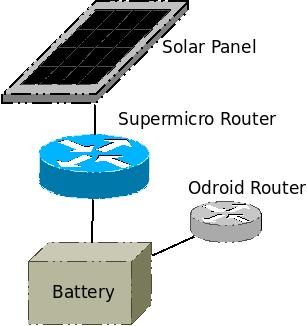
\includegraphics[width=\textwidth]{wire_odroid.jpeg}
\caption{Supermicro and Odroid routers share the power supply system}
\end{subfigure}
\begin{subfigure}{0.45\textwidth}
\centering
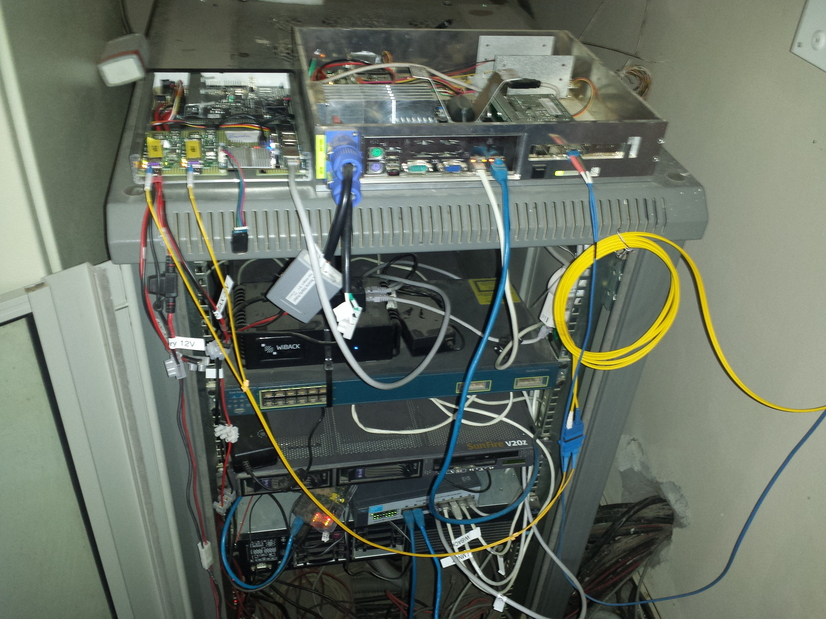
\includegraphics[width=\textwidth]{bunda_sbstn.jpg}
\caption{Equipments at Bunda substation}
\end{subfigure}
\caption{Cable solution of Supermicro and Odroid routers to share power supply system}
\label{wiring}
\end{figure}